\documentclass[10pt,superscriptaddress,
amsmath,aps,prc,twocolumn,nofootinbib,floatfix]{revtex4-1}
\ifdefined\DeclareUnicodeCharacter
  \DeclareUnicodeCharacter{03C9}{$\omega$}
  \DeclareUnicodeCharacter{03C3}{$\sigma$}
\fi

\usepackage{amssymb}  % \gtrsim, \geqslant, etc: see amsguide.ps
\usepackage{graphicx}
\usepackage{exscale}
\usepackage{textcomp}
\usepackage{enumerate}
%\usepackage[spanish]{babel}
\usepackage{amsmath}
\usepackage{empheq}
\usepackage{amssymb}
%\usepackage[compat=1.1.0]{tikz-feynhand} 
\usepackage{multirow}
\usepackage{orcidlink}
%\usepackage{float}
\usepackage{subcaption}
\usepackage{float}
%\usepackage{cite}
%\usepackage{bm}
% \addtolength{\topmargin}{2cm}
%\usepackage[utf8]{inputenc}
%\usepackage[T1]{fontenc}

%%%%%%%%%%%%%%%%%%%%%%%%%%%%%%%%%%%%%%%%%%%%%%%%%%%%%%%%%%%%%%%%%
%%    This is our standard definitions of abbreviations        %%
%%%%%%%%%%%%%%%%%%%%%%%%%%%%%%%%%%%%%%%%%%%%%%%%%%%%%%%%%%%%%%%%%

\usepackage{color}
\newcommand{\com}[1]{{\sf\color[rgb]{0,0,1}[#1]}}
% Marking old and new text:
\usepackage[normalem]{ulem}  % \sout{old text} for strikeout
\newcommand{\mga}[1]{{\color[rgb]{0.8,0,0}#1}}
\newcommand{\mgacom}[1]{\textsf{\color[rgb]{0.7,0,0}[\textsuperscript{MGA} #1]}}
%\newcommand{\new}[1]{#1}
\newcommand{\old}[1]{{\color[rgb]{0.7,0.7,0.7}\sout{#1}}}
\newcommand{\new}[1]{{\color[rgb]{0.7,0,0.7}#1}}

\newcommand{\AH}[1]{{\color{cyan}#1}}
\newcommand{\AHcom}[1]{\textsf{\color{cyan}{\textsuperscript{AH}#1}}}

\newcommand{\LB}[1]{{\color{brown}#1}}
\newcommand{\LBcom}[1]{\textsf{\color{brown}[\textsuperscript{LB}#1]}}

\newcommand{\JS}[1]{{\color{violet}#1}}
\newcommand{\JScom}[1]{\textsf{\color{violet} [\textsuperscript{JS}#1]}}

%%%%%%%%%% Journal Styles for APS
%\newcommand\NCA{Nuovo Cimento}
%\newcommand\NPBPS{{Nucl. Phys.} B (Proc. Suppl.)}
%\newcommand\RMP{Rev. Mod. Phys.}
%\newcommand\PTP{{Prog. Theor. Phys.}}
%\newcommand\PTPS{{Prog. Theor. Phys. Suppl.}}
%\newcommand\ZPA{{Z. Phys.} A}
%\newcommand\EPJA{{Eur. Phys. J.} A}
\newcommand{\AP}[3]{Ann.\ Phys.\ {\bf #1},\ #2 (#3)}
\newcommand{\NPA}[3]{Nucl.\ Phys.\ {\bf A#1},\ #2 (#3)}
\newcommand{\NPB}[3]{Nucl.\ Phys.\ {\bf B#1},\ #2 (#3)} 
\newcommand{\PLA}[3]{Phys.\ Lett.\ A\ {\bf #1},\ #2 (#3)}
\newcommand{\PLB}[3]{Phys.\ Lett.\ B\ {\bf #1},\ #2 (#3)}
\newcommand{\PR}[3]{Phys.\ Rep.\ {\bf #1},\ #2 (#3)}
\newcommand{\PRL}[3]{Phys.\ Rev.\ Lett.\ {\bf #1},\ #2 (#3)}
\newcommand{\PRB}[3]{Phys.\ Rev.\ B\ {\bf #1},\ #2 (#3)}
\newcommand{\PRC}[3]{Phys.\ Rev.\ C\ {\bf #1},\ #2 (#3)}
\newcommand{\PRD}[3]{Phys.\ Rev.\ D\ {\bf #1},\ #2 (#3)}
\newcommand{\JPG}[3]{J.\ Phys.\ G\ {\bf #1},\ #2 (#3)}
\newcommand{\RPP}[3]{Rep.\ Prog.\ Phys.\ {\bf #1},\ #2 (#3)}
\newcommand{\ZPC}[3]{Z.\ Phys.\ C\ {\bf #1},\ #2 (#3)}
\newcommand{\EPJC}[3]{Eur.\ Phys.\ J.\ C\ {\bf #1},\ #2 (#3)}
\newcommand{\PPNP}[3]
{Prog.\ Part.\ Nucl.\ Phys.\ {\textbf #1},\ #2 (#3)}
\newcommand{\APPB}[3]{Acta.\ Phys.\ Polon.\ B\ {\bf #1},\ #2 (#3)}

\newcommand{\ibid}[3]{{\bf #1},\ #2 (#3)}
%%%%%%%%%% End Journal Definitions

%%%%%%%%%% Greek alphabets
\renewcommand\a{\alpha}
\renewcommand\b{\beta}
\newcommand\g{\gamma}
\renewcommand\d{\delta}
\newcommand\e{\epsilon}
\newcommand\ve{\varepsilon}
\newcommand\z{\zeta}
\newcommand\h{\eta}
\newcommand\q{\theta}
\renewcommand\i{\iota}
\renewcommand\k{\kappa}
\renewcommand\l{\lambda}
%\newcommand\m{\mu}
\newcommand\n{\nu}
\newcommand\x{\xi}
%\newcommand\p{\pi}
\newcommand\rr{\rho}
%\newcommand\s{\sigma}
\renewcommand\t{\tau}
\renewcommand\u{\upsilon}
\newcommand\f{\phi}
\renewcommand\c{\chi}
\renewcommand\j{\psi}
\renewcommand\o{\omega}

\newcommand{\al}{\alpha}
\newcommand{\be}{\beta}
\newcommand{\ga}{\gamma}
\newcommand{\Ga}{\Gamma}
\newcommand{\de}{\delta}
\newcommand{\De}{\Delta}
\newcommand{\ep}{\varepsilon}

\newcommand{\eps}{\epsilon}
\newcommand{\ze}{\zeta}
\newcommand{\ka}{\kappa}
\newcommand{\la}{\lambda}
\newcommand{\La}{\Lambda}
\newcommand{\ph}{\varphi}
\newcommand{\del}{\nabla}
\newcommand{\si}{\sigma}
\newcommand{\Si}{\Sigma}
\renewcommand{\th}{\theta}   % LaTeX: \th already defined
\newcommand{\Up}{\Upsilon}
\newcommand{\om}{\omega}
\newcommand{\Om}{\Omega}

%%%%%%%%%% End Greek alphabets

%%%  A few capitals
\newcommand\D{\Delta}
\newcommand\G{\Gamma}
\renewcommand\L{\Lambda}
\newcommand\J{\Psi}
\newcommand\U{\Upsilon}

%%%%%%%%%%  Some abbreviations

%\newcommand{\Del}{\nabla}
%\newcommand{\eqn}[1]{(\ref{#1})}
%\newcommand{\sliver}{\kern 0.07em} % like italic correction \/

\newcommand{\m}{\text{m}}
\newcommand{\km}{\text{km}}
\newcommand{\s}{\text{s}}
\newcommand{\gram}{\text{g}}
\newcommand{\MeV}{\text{MeV}}
\newcommand{\kHz}{\text{kHz}}
\newcommand{\nsat}{\ensuremath{n_{0}}}
\newcommand{\Qstar}{\ensuremath{Q^*}}
\newcommand{\N}{{\ensuremath{N}}}
\newcommand{\Nbar}{{\ensuremath{\bar N}}}
\newcommand{\Qbar}{{\ensuremath{\bar Q}}}

\newcommand{\Bratio}{\lambda_n}
\newcommand{\tfinal}{\ensuremath{t_\text{eq}}}

%\newcommand{\half} {{\textstyle \frac{1}{2}}}
%\newcommand\deriv[3]{{\dfrac{\partial #1}{\partial #2}}\biggr|_{#3}}
%\newcommand{\p}{\partial}


\begin{document}

\title{Quark Matter Phase Boundary Evolution in Neutron Star Mergers}
 \author{M.~G.~Alford \,\orcidlink{0000-0001-9675-7005}}
 \email{alford@physics.wustl.edu}
 \affiliation{Department of Physics, Washington University in St.~Louis, St.~Louis, MO 63130, USA}
 \author{L.~Brodie\,\orcidlink{0000-0001-7708-2073}}
 \email{b.liam@wustl.edu}
 \affiliation{Department of Physics, Washington University in St.~Louis, St.~Louis, MO 63130, USA}
 \author{A.~Haber\,\orcidlink{0000-0002-5511-9565}}
 \email{a.haber@soton.ac.uk}
 \affiliation{Mathematical Sciences and STAG Research Centre,
University of Southampton, Southampton SO17 1BJ, United Kingdom}
 \affiliation{Department of Physics, Washington University in St.~Louis, St.~Louis, MO 63130, USA}
 \author{J. Shao\,\orcidlink{0009-0004-9698-0177}}
 \email{jan.shao@wustl.edu}
 \affiliation{Department of Physics, Washington University in St.~Louis, St.~Louis, MO 63130, USA}
 \affiliation{McDonnell Center for the Space Sciences, Washington University in St.~Louis, St.~Louis, MO 63130, USA}

\date{\today}

\begin{abstract}
Place holder
\end{abstract}

\maketitle

\section{Introduction}

Neutron star mergers provide a rare opportunity to study the dynamics of neutron star matter on the millisecond timescale. It is hoped that this information will help us to map the phases of ultra-dense matter. For example, if there were a first-order phase transition from nuclear matter to quark matter at some critical pressure, would it produce observable signatures in the gravitational or electromagnetic waves emitted, either during the inspiral or after the merger? In both scenarios, the speed at which the boundary moves is an essential factor.

\AH{In the inspiral phase, \mga{a phase boundary between nuclear and quark matter
can create observable signatures via excitation of its ``interface mode'' \cite{Counsell:2025hcv,Pereira:2025xsi}.
Such excitations,}
%this transition from nuclear matter to quark matter could lead to the excitation of the so-called interface mode. This interface mode, 
which would provide strong evidence for the existence of quark matter, are potentially detectable with the current LVK network, and certainly within reach of next-generation detectors like Cosmic Explorer or the Einstein Telescope \cite{Counsell:2025hcv,Pereira:2025xsi}. However, the existence and frequency of the interface mode critically depend on the conversion timescale, i.e.,~the speed with which the phase boundary between nuclear and quark matter can move \mga{via conversion of metastable nuclear matter to quark matter, or vice versa}. If the phase boundary can move too fast, the restoring force for the interface mode and thus the mode itself vanish. All recent analyses %\mgacom{citation}
\cite{Tonetto:2020bie,Counsell:2025hcv,Pereira:2025xsi} thus set this velocity to zero and assume that on the millisecond timescale of the oscillation, the phase content is frozen.}

\mga{In the post-merger phase there are also possible signatures of
a nuclear-quark phase boundary.}
Several recent works have addressed this question using model equations of state that include a nuclear/quark transition \cite{Most:2018eaw,Bauswein:2018bma,Espino:2023llj,Weih:2019xvw,Harada:2023eyg,Bauswein:2020ggy,Haque:2022dsc,Fujimoto:2022xhv,Christian:2023hez,Fujimoto:2024ymt},
\mga{looking for features of the gravitational wave emission arising}
from the redistribution of mass
as regions of the denser phase grow or shrink in response to pressure gradients in the violent collision between the stars. 
Current simulations assume that if a region of nuclear matter is compressed to a pressure above the critical pressure $p_\text{crit}$ where quark matter becomes favored, it will immediately convert to quark matter,
%If we neglect the problem of nucleating the new phase, and assume that there is already a neighboring region of quark matter, then the conversion occurs by the quark matter phase growing and consuming the (now metastable) nuclear matter. 
so there will be no significant regions of metastable nuclear matter
\mga{or out-of-equilibrium quark matter}. This assumes that the phase boundary can travel distances of order kilometers in milliseconds, i.e., at speeds of order $10^6\,\m\s^{-1}$. However, it is known that since weak interactions are required to create strange quarks, the boundary speed is limited.

%as noted in the earliest work on the formation of strange stars \cite{Olinto:1986je},  conversion of nuclear matter to quark matter requires weak interactions to create strange quarks, so there will be a limit on how fast the conversion of one phase to another can occur. 

In this Letter, we estimate how fast a region of metastable nuclear matter could be converted to quark matter \mga{via a deflagration arising from a gradual (compared to microscopic timescales) increase in pressure  \mgacom{Need to say how our work relates to these previous ones:} \cite{Olinto:1986je,Niebergal:2010ds,Furusawa:2015vfn,Drago:2015fpa}. Detonation-type conversion induced by a shock is a separate phenomenon \cite{Furusawa:2015gjj} whose treatment we defer to future work.}
\mgacom{This is the minimal treatment. We could get in to a discussion of when detonation is physically realized, but for that we'd have to understand the physics better.}\JScom{Relate what we are doing with what have been done, what makes our work necessary. }

We first estimate the maximum speed at which the phase boundary could travel, and then the timescale on which the boundary will reach its equilibrium position. We find that the speeds are generally slow on the timescale of a merger, leading us to conclude that \mga{post-merger} simulations of matter with such transitions should take into account the finite speed of the boundary. 
\mga{For the inspiral phase, the speed may be slow enough to allow} interface modes. \mgacom{Moved discussion of phase conversion dissipation to the conclusions}
We do not consider the reverse process, conversion of quark matter to nuclear matter, %\AH{and the calculation of the phase conversion dissipation,} 
leaving that to future work.\LBcom{Should we also move this to the conclusions, where we can also mention including hyperons?}
We use natural units, $\hbar=c=k_B=1$.


%\JScom{Could add this to address Furusawa and Ouyed?}
%\JS{Previous studies of hadron–quark conversion in compact stars have largely focused on shock- or hydrodynamically driven scenarios, where the propagation speed of the conversion front is determined by global fluid dynamics rather than by microphysics alone. In this context, reactive hydrodynamical analyses have classified possible combustion modes using Hugoniot constructions and have demonstrated that detonation-like conversion may occur under sufficiently strong compression. Complementary numerical studies have explored such scenarios in proto-neutron stars and quark-nova models using dedicated hydrodynamical codes.

%However, these approaches typically assume the presence of strong hydrodynamic forcing and do not address the limiting case in which the conversion proceeds without shocks or externally imposed compression. In particular, the conversion speed is often treated as an input or emergent hydrodynamical parameter rather than being derived from microphysical transport and weak interaction rates. In contrast, neutron-star mergers generically contain extended regions that evolve quasi-hydrostatically after the initial collision, where such forcing may be absent. In this work, we therefore focus on the diffusion-limited regime and derive conservative, microphysics-based bounds on the conversion speed, independent of assumptions about shock formation or large-scale fluid dynamics.}

\section{Methods}
\label{sec:hydro_methods}

We estimate the steady propagation speed of the phase boundary that converts metastable nuclear matter into strange quark matter.  
The nuclear phase is modeled as pure neutron matter described by the QMC-RMF3 equation of state~\cite{Alford:2022bpp,Alford:2023rgp,qmc_rmf3}.  The quark phase is treated as degenerate gas of massless \mga{noninteracting} up, down, and strange quarks with a bag constant~\cite{Chodos:1974je,Farhi:1984qu}.  
We assume that the surface tension is large enough to exclude a spatially extended mixed phase and that the conversion proceeds as a deflagration. \JScom{Do we still need this assumption in our new setting? I remember we assume this because before, we didn't model udQM in our previous picture, but I think the quark EoS now can describe non-leptonic udQM.} 
The front is taken to be 1-dimensional because the conversion layer is microscopic compared with the macroscopic length scales of a neutron star. \mgacom{Also we neglect any instabilities that might lead to "mushrooming" or "fingering" structures.}

\mgacom{The broad description should come here, and it would work better as a description of a schematic figure}
We work in the rest frame of the interface, placed at $x=0$.  Nuclear matter flows toward the interface from $x<0$, and quark matter flows away from it through $x>0$. 
We label the homogeneous nuclear state immediately ahead of the interface by $\N$, the just-deconfined quark state at $x=0^+$ by $\Qstar$, and the flavor-equilibrated quark state at $x\to\infty$ by $\Qbar$.  Superscripts
or subscripts carrying one of these labels indicate the state at which a
quantity is evaluated.  Thus, for example, $n_B^\N$ and $u_\N$ belong to
the nuclear state, whereas $n_B^{\Qstar}$ and $u_{\Qstar}$ are their values just
behind the interface.  \mgacom{Is it clear that we need to use the labels $\Qstar$ etc rather than $a(0^+), n_B(0^+)$ etc?}
%Deconfinement at the interface occurs on the strong-interaction timescale.  

Flavor equilibration behind the interface is slower and is governed by the nonleptonic process $d u\leftrightarrow u s$.  
We neglect electrons, electromagnetism, and Urca reactions, since Urca processes are slower than the nonleptonic channel in the regime of interest\cite{Alford:2006gy,Alford:2025tbp,Sad:2007afd}, this omission is consistent with seeking an upper estimate of the conversion speed.

Deconfinement at the sharp interface occurs through strong interactions and is
therefore fast compared with flavor equilibration. Therefore, nuclear matter arriving at the boundary can convert immediately into a nonequilibrated quark
state $\Qstar$, which already contains some strangeness from diffusion, but has not reached the
flavor composition of $\Qbar$.  On the quark side, the nonleptonic reaction
$d u\leftrightarrow u s$ relaxes the flavor imbalance while the associated
concentration gradient diffuses strangeness toward the interface.  The
combination of weak conversion and diffusion determines the steady boundary
speed.

The composition variable transported through the quark conversion layer is the \mga{imbalance between the $d$ and $s$ quark densities which we call ``K''
since it has the quantum numbers of a Kaon,} \mgacom{Let's talk in terms of K-ness rather than Kaon-ness since people will think we mean actual Kaon particles.}\JScom{addressed}
\begin{equation}
 n_K \equiv \frac{n_d-n_s}{2}\ ,
 \qquad
 \mu_K\equiv\mu_d-\mu_s\ .
\label{eq:hydro_nK_definition}
\end{equation}
\mgacom{Please note that we need to put a space between an equation and the following punctuation mark, e.g.:}~\verb!\mu_d-\mu_s\ .!
\AHcom{we normally use half spaces: backslash comma}
Here $n_i$ and $\mu_i$ denote the number density and chemical potential of quark flavor $i$:

For the massless-quark model used here, flavor equilibrium in $\Qbar$ implies
$n_K^{\Qbar}=\mu_K^{\Qbar}=0$.
We define the local $K$ fraction by
\begin{equation}
 a(x)\equiv\frac{n_K(x)}{n_B(x)}\ ,
 \quad
 a_{\Qstar}\equiv a(0^+) \ ,
 \quad
 a_{\Qbar}\equiv a(\infty)=0\ .
\label{eq:hydro_a_definition}
\end{equation}
%so that both densities entering the fraction are evaluated at the same position.  
Here $a_{\Qstar}$ is the $K$ fraction immediately behind the interface.  
In pure neutron matter $n_K^N=n_B^N$, so the corresponding $K$ fraction in pure neutron matter is \mga{
\begin{equation} 
a_N\equiv a(0^-)=1 \ .
\end{equation}
}

Figure~\ref{fig:hydro_example_profile} is an example of $K$-ness fraction, temperature, velocity field, and baryon number density profiles. The nuclear state is uniform for $x<0$.  Strong deconfinement
produces discontinuities in the thermodynamic and hydrodynamic variables at
$x=0$, after which $a(x)$ relaxes smoothly from $a_{\Qstar}$ to zero in the
quark matter side.  The temperature approaches its downstream value on
the same microscopic scale, whereas the relative changes of $u$ and $n_B$
within the quark matter side are too small to see at the plotted resolution.

\begin{figure*}[t]
  \centering
  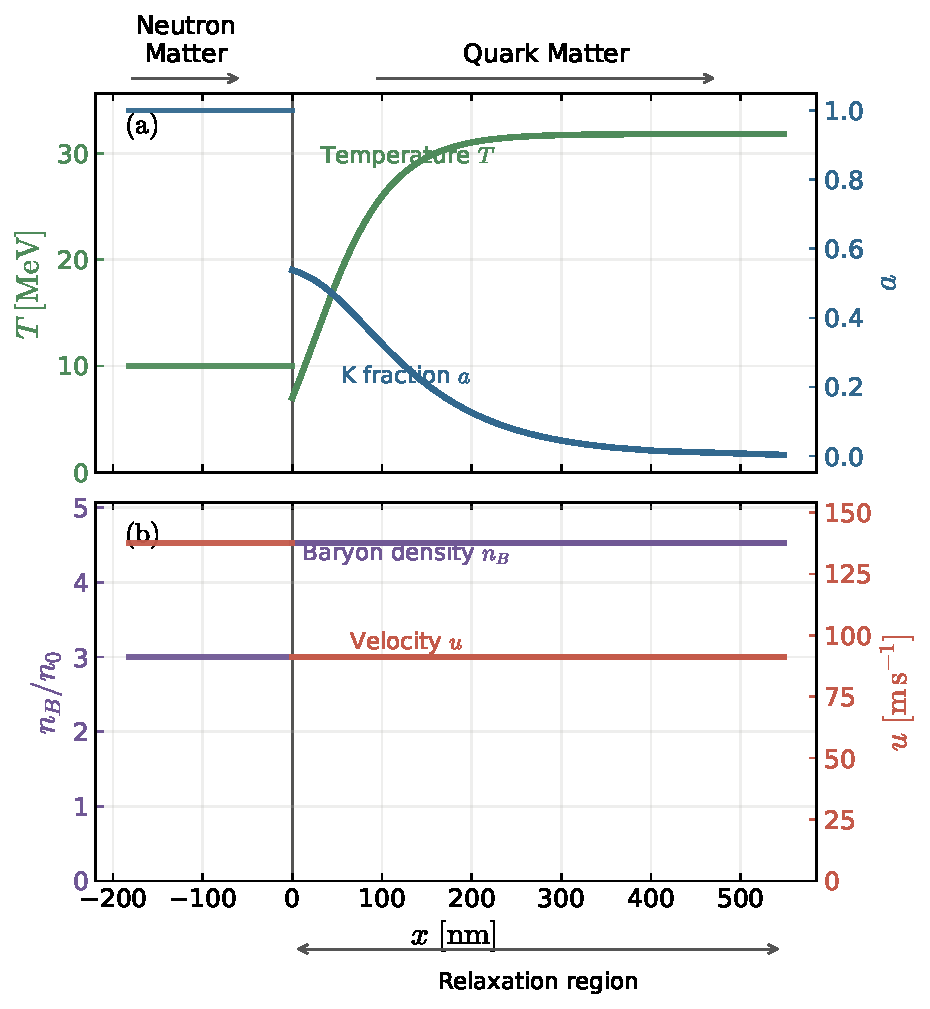
\includegraphics[width=0.8\textwidth]{Plots/Example_profile.pdf}%
  \caption{Representative energy-conserving conversion-front solution for
  $T_N=10~{\rm MeV}$, $B^{1/4}=180~{\rm MeV}$,
  $n_B^N=3n_0$, and $a_{\Qstar}=0.55$.  The dashed segments show the uniform
  nuclear state at $x<0$ \mgacom{Do we need to make it dashed?}\JScom{Now un-dashed} , the solid curves show the quark phase at $x>0$, and
  the vertical line marks the interface.  The panels show (a) the local K-
  fraction, (b) the fluid velocity, (c) the temperature, and (d) the baryon
  density.}
  \label{fig:hydro_example_profile}
\end{figure*}

For completeness, we first state the relativistic steady-front equations.  
The energy density, pressure, four-velocity, and baryon density are denoted by $\epsilon$, $P$, $U^\mu$, and $n_B$, respectively.  
The perfect-fluid stress tensor and baryon current are
\begin{equation}
 T^{\mu\nu}=h U^\mu U^\nu+P g^{\mu\nu},
 \qquad
 N_B^\mu=n_B U^\mu,
\label{eq:hydro_stress_tensor}
\end{equation}
where $h=\epsilon+P$ is the enthalpy density.  Writing the four-velocity as $U^\mu=(\gamma,u,0,0)$, with
\begin{equation}
 \gamma=(1-v^2)^{-1/2},
 \qquad
 u=\gamma v,
\label{eq:hydro_lorentz_factor}
\end{equation}
The solutions considered below satisfy $v\ll1$.  In the analytical
approximation we therefore set $\gamma=1$ and identify $u=v$.  The numerical
calculation retains the exact relation $\gamma=\sqrt{1+u^2}$.
We assume the phase boundary moves in a deflagration and stationary manor, and with planar symmetry, which reduce baryon conservation $\partial_\mu N^\mu = 0$ and energy-momentum conservation $\partial_\mu T^{\mu\nu} = 0$ to one-dimensional flux equations.  
Including $K$ diffusion and the weak source gives
\begin{subequations}
\label{eq:hydro_front_system}
\begin{empheq}[left=\empheqlbrace]{align}
 &\frac{d}{dx}\left(u n_B\right)=0,
\label{eq:hydro_baryon_conservation}\\
&\frac{d}{dx}\left(h u\right)=0,
\label{eq:hydro_energy_conservation}\\
 &\frac{d}{dx}\left(h u^2+P\right)=0,
\label{eq:hydro_momentum_conservation}\\
&\frac{d}{dx}\left(u n_K-D_K\frac{dn_K}{dx}\right)
=-\Gamma_K.
\label{eq:hydro_K-_conservation}
\end{empheq}
\end{subequations}
Here $\Gamma_K$ is the positive weak relaxation rate that depletes $K$ density and $D_K$ is the flavor-diffusion coefficient. 
Integrating Eqs.~\eqref{eq:hydro_front_system} across the sharp interface yields the hydrodynamic jump conditions across the phase boundary:
\begin{subequations}
\label{eq:hydro_jump_conditions}
\begin{empheq}[left=\empheqlbrace]{align}
 &n_B^N u_N=n_B^{\Qstar}u_{\Qstar},
\label{eq:hydro_jump_baryon}\\
 &h_Nu_N=h_{\Qstar}u_{\Qstar},%\gamma_{\Qstar},
\label{eq:hydro_jump_energy}\\
 &h_Nu_N^2+P_N=h_{\Qstar}u_{\Qstar}^2+P_{\Qstar},
\label{eq:hydro_jump_momentum}\\
 &u_{\Qstar}n_K^{\Qstar}
 -D_K^{\Qstar}\left.\frac{dn_K}{dx}\right|_{0^+}
 =u_Nn_K^N.
\label{eq:hydro_jump_K-}
\end{empheq}
\end{subequations}
The four lines impose continuity of baryon, energy flux, momentum flux, and $K$-ness, respectively.
The $K$ condition contains no diffusive term on the homogeneous nuclear side.  

For positive $\mu_K$, the nonleptonic process relaxes the $K$ density at the
rate~\cite{Madsen:1993xx}
\begin{equation}
 \Gamma_K(\mu_B,\mu_K,T)
 =\mathcal A_K\mu_u^5\mu_K
 \left(\mu_K^2+4\pi^2T^2\right),
\label{eq:hydro_exact_rate}
\end{equation}
where $\mu_K=\mu_d-\mu_s$.  The exact weak prefactor is
\begin{equation}
 \mathcal A_K=
 \frac{16}{5\pi^5}G_F^2
 \sin^2\theta_C\cos^2\theta_C,
\label{eq:hydro_exact_prefactor}
\end{equation}
where $G_F$ is the Fermi constant and $\theta_C$ is the Cabibbo angle.  We use
$\mu_u=\mu_B/3+2\mu_Q/3$, where electric charge chemical potential $\mu_Q$ is fixed by charge neutrality,
$2n_u-n_d-n_s=0$.
We use the perturbative diffusion coefficient~\cite{Haensel:1992zz}
\begin{equation}
 D_K^{-1}
 =
 \frac{8N_f\alpha_s^2}{\pi}
 \left(
 h_D\frac{T^{5/3}}{q_D^{2/3}}
 +\frac{\pi^3T^2}{12q_D}
 \right),
\label{eq:hydro_diffusion_coefficient}
\end{equation}
Here $N_f=3$ is the number of active quark flavors, $\alpha_s$ is the strong coupling, $h_D = \Gamma(\frac{8}{3})\zeta(\frac{5}{3})(2\pi)^{2/3} \simeq1.81$ is a numerical prefactor, $q_D$ is the
Debye wavenumber defined by $q_D^2=g^2N_f\mu_q^2/(2\pi^2)$, and $g^2=4\pi\alpha_s$.
The physical $K$ current, directed toward increasing $x$, is
\begin{equation}
 j_K(x)\equiv
 u(x)n_K(x)-D_K(x)\frac{dn_K}{dx}.
\label{eq:hydro_jK_definition}
\end{equation}
Equation~\eqref{eq:hydro_K-_conservation} can therefore also be written as
$dj_K/dx=-\Gamma_K$.\JScom{State the task: solve Eq.~\eqref{eq:hydro_K-_conservation}}

\subsection{Piecewise-constant analytical approximation}
\label{sec:hydro_analytic}

\JScom{State the approximation first then say why it's a good approximation}
To understand Eq.~\eqref{eq:hydro_front_system}, we first adopt an approximation to get some analytical results. 
For massless quarks close to flavor equilibrium, at leading order in
$\mu_K/\mu_q$ and $T/\mu_q$, where $\mu_q=\mu_B/3$, the charge-neutral quark
equation of state gives
\begin{equation}
 \mu_u\simeq\mu_q,
 \qquad
 n_B\simeq\frac{\mu_q^3}{\pi^2},
 \qquad
 \mu_K\simeq\frac{2}{3}\mu_q a.
\label{eq:hydro_cubic_rate_expansion}
\end{equation}
Substituting Eq.~\eqref{eq:hydro_cubic_rate_expansion} into the exact rate in
Eqs.~\eqref{eq:hydro_exact_rate} and \eqref{eq:hydro_exact_prefactor}, and
retaining the leading cubic and thermal-linear terms, gives \JScom{This rate Eq. is not specific for the piecewise constant approximation}
\begin{subequations}
\label{eq:hydro_cubic_rate}
\begin{align}
 \Gamma_K(n_K,T)
 &=n_B\gamma_K\left(a^3+\eta a\right),
 \qquad
 \eta=\frac{9\pi^2T^2}{\mu_q^2},
\label{eq:hydro_source}\\
 \gamma_K
 &=\frac{128}{27\times5\pi^3}
 G_F^2\sin^2\theta_C\cos^2\theta_C\,\mu_q^5.
\label{eq:hydro_gammaK}
\end{align}
\end{subequations}
\AHcom{rates in terms of mu or a?}
The approximation is controlled by the separation between the microscopic conversion width and the hydrodynamic scale height \mgacom{``scale height'' sounds like a term from planetary physics... and I'm not sure what we are describing anyway.}.  
Balancing flavor diffusion against the local weak source gives the characteristic weak relaxation time $\tau_{\rm weak}$ and conversion-layer thickness
$L_{\rm weak}$:
\begin{align}
 \tau_{\rm weak}&\sim
 \frac{1}{\gamma_K(a^2+\eta)},
\notag\\
 L_{\rm weak}\sim
 \sqrt{D_K\tau_{\rm weak}}
 &=
 \left[\frac{D_K}{\gamma_K(a^2+\eta)}\right]^{1/2}.
\label{eq:hydro_weak_length}
\end{align}
\mgacom{Where did this come from?}
%This estimate is dimensionally consistent in natural units:
%$D_K$ and $\tau_{\rm weak}$ both have dimension ${\rm energy}^{-1}$, or equivalently length, whereas $\gamma_K$ has dimension energy.  Thus $D_K\tau_{\rm weak}$ has dimension length squared.
%Restoring $c$, the conventional diffusion coefficient is $cD_K$ and has dimension length squared per unit time.
For $\alpha_s=0.3$, $\mu_q=300$--$400~{\rm MeV}$,
$T=1$--$50~{\rm MeV}$, and order-unity composition,
$\tau_{\rm weak}$ is of order nanoseconds and $L_{\rm weak}$ ranges from tens of nano-meters to a few micrometers.  
By contrast, a representative stellar gradient $\lvert dn_B/dz\rvert\sim0.3n_0\,{\rm km}^{-1}$ at $n_B\sim3n_0$ corresponds to a density scale height of about $10~{\rm km}$.  
The expected fractional change in $n_B$ across the conversion layer is therefore at most of order $10^{-10}$, and the pressure scale is comparable.  Momentum conservation gives the same conclusion locally: the departure from constant pressure is of relative order $(h/P)u^2$, while the weak-diffusive estimate $u\sim[D_K\gamma_K(a^2+\eta)]^{1/2}$ is sub-kilometer per second and hence $u^2\lesssim10^{-11}$ in natural units.

\mgacom{We should describe our approx at the start, and then justify it.}
Therefore, we treat quantities $T(x)$, $\mu_K(x)$, $n_K(x)$, and $a(x)$ are varying profiles on the quark side, running from $\Qstar$ at $x=0^+$ to $\Qbar$ at $x\to\infty$, and any other quantities, such as $P, n_B, \mu_B, h$, etc. as piecewise constant.
We therefore write the varying quantities without a $\Qstar$ or $\Qbar$ label except when referring specifically to an endpoint; the endpoint labels do not denote different profile functions.  
By contrast, a bare $Q$ labels the piecewise constant quantities treated throughout the quark matter side in this approximation, such as $n_B^Q$, $u_Q$, and $\mu_B^Q$.

We therefore hold $n_B$, $u$, $\mu_B$, and $P$ fixed within each phase, while retaining the spatial variation of $n_K$, $a$, $\mu_K$, and $T$.  
Since $n_K^N=n_B^N$ in pure neutron matter, define $\Bratio$ as the baryon number density ratio across the phase boundary, the baryon conservation across the phase boundary gives
\begin{equation}
 \Bratio \equiv\frac{n_B^N}{n_B^Q}
 =\frac{n_K^N}{n_B^Q},
 \qquad
 u_Q=\Bratio u_N,
\label{eq:hydro_piecewise_flux}
\end{equation}
where the second relation follows from baryon-flux conservation.  
On the quark side,
\begin{equation}
 j_K=n_B^Q\left(u_Qa-D_Ka'\right),
 \qquad
 \frac{dj_K}{dx}
 =-n_B^Q\gamma_K\left(a^3+\eta a\right).
\label{eq:hydro_piecewise_transport}
\end{equation}
Current matching gives $j_K(0^+)=u_Nn_B^N=u_Qn_B^Q$, and therefore
\begin{equation}
 D_K(T_{\Qstar})a'(0^+)
 =-\Bratio u_N(1-a_{\Qstar}).
\label{eq:hydro_interface_gradient}
\end{equation}

We now follow the Olinto construction used for a diffusion-limited front 
\mgacom{We can say when our results agree with Olinto but let's not seem to be ``following'' her, we are doing a much better calcualtion.} \cite{Olinto:1986je}.  Dividing Eq.~\eqref{eq:hydro_piecewise_transport} by $n_B^Q$ gives
\begin{equation*}
 \frac{d}{dx}\left(D_Ka'\right)
 =u_Qa'+\gamma_K\left(a^3+\eta a\right).
\end{equation*}
Multiplying by $D_Ka'$, integrating from $0^+$ to the equilibrated state, and using Eq.~\eqref{eq:hydro_interface_gradient} gives the balance
\begin{equation*}
 -\frac{1}{2}
 \left[\Bratio u_N(1-a_{\Qstar})\right]^2
 =
 u_Q\int_0^\infty D_K(a')^2\,dx-I,
\end{equation*}
where $I$ is defined below in Eq.~\eqref{eq:hydro_I_definition}.
The remaining profile integral can be written without specifying the full solution.  
For the monotonic front profiles of interest, we assume that $D_Ka'$ lies between $-\Bratio u_N(1-a_{\Qstar})$ at the interface and zero downstream.  %==============
We therefore parameterize its weighted mean directly by
$\xi$:
\begin{equation*}
 \int_0^\infty D_K(a')^2\,dx
 =
 \frac{1+\xi}{2}\,
 \Bratio u_N(1-a_{\Qstar})a_{\Qstar}.
\end{equation*}
Here $-1<\xi<1$ characterizes the shape of the diffusion profile. 
Substituting this relation into the balance yields
\begin{align}
 u_N^2&=
 \frac{2I}
 {\Bratio^2(1-a_{\Qstar})(1+\xi a_{\Qstar})},
\label{eq:hydro_speed_general}\\
 I&\equiv
 \gamma_K\int_0^{a_{\Qstar}}
 D_K(T(a))\left[a^3+\eta(T(a))a\right]\,da,
\label{eq:hydro_I_definition}
\end{align}

To evaluate the integral Eq.~\eqref{eq:hydro_I_definition}, at fixed $\mu_B=3\mu_q$, the leading terms of $\mu_K$ and $T$ in the bag-model pressure give
\begin{equation}
 P_{\rm QM}(\mu_B,\mu_K,T)-P_{\rm QM}(\mu_B,0,0)
 \simeq
 \frac{\mu_B^2\mu_K^2}{12\pi^2}
 +\frac{\mu_B^2T^2}{6}.
\end{equation}
Here the omitted terms are quartic in $\mu_K$ and $T$.
For the profiles considered here, $\mu_K/\mu_B\lesssim0.12$ and $T/\mu_B\lesssim0.03$, so the pure $\mu_K^4$ correction is below $1\%$ and the thermal and mixed quartic corrections remain at the few-percent level.
Comparing any point on the isobar with the equilibrated downstream state, where $\mu_K=0$ and $T=T_{\Qbar}$, therefore gives
\begin{equation}
 T^2+\frac{\mu_K^2}{2\pi^2}=T_{\Qbar}^2.
\end{equation}
In addition, since
\begin{equation}
 n_K=
 \left(\frac{\partial P_{\rm QM}}{\partial\mu_K}\right)_{\mu_B,T}
 \simeq\frac{3\mu_q^2\mu_K}{2\pi^2},
 \qquad
 n_B\simeq\frac{\mu_q^3}{\pi^2}.
\end{equation}
Thus $a=n_K/n_B\simeq3\mu_K/(2\mu_q)$, or $\mu_K\simeq(2/3)\mu_q a$.  
Defining $A$ by the zero-temperature endpoint of the same isobar,
$A^2=9\pi^2T_{\Qbar}^2/(2\mu_q^2)$, yields
\begin{equation}
 T^2(a)=\frac{2\mu_q^2}{9\pi^2}(A^2-a^2),
 \qquad
 \eta(a)=2(A^2-a^2),
\label{eq:hydro_constant_pressure_path}
\end{equation}
where the second relation follows from
$\eta=9\pi^2T^2/\mu_q^2$.  
Since $\mu_K$ is proportional to $a$ at this order, Eq.~\eqref{eq:hydro_constant_pressure_path} is the same quarter ellipse in either the $(\mu_K,T)$ or $(a,T)$ plane.

\begin{figure}[t]
  \centering
  \IfFileExists{Plots/T_a_constant_pressure.pdf}{%
    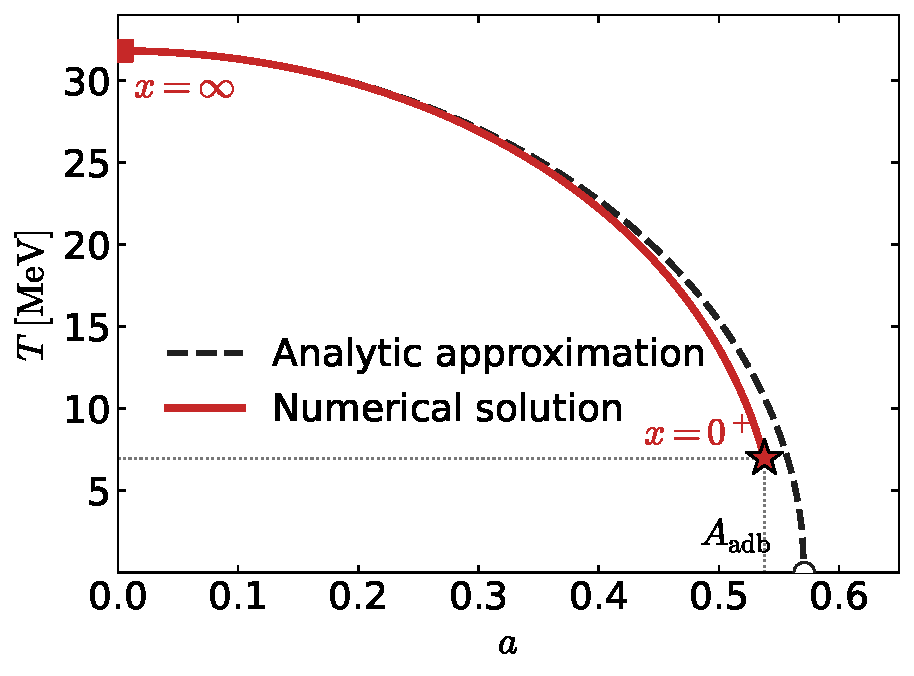
\includegraphics[width=\columnwidth]{Plots/T_a_constant_pressure.pdf}%
  }{%
    \includegraphics[width=\columnwidth]{Hydrodynamical combustion/Plots/T_a_constant_pressure.pdf}%
  }
  \caption{Constant-pressure trajectory through the quark conversion layer.
  The red curve is the energy-conserving numerical profile for
  $T_N=10~{\rm MeV}$, $B^{1/4}=180~{\rm MeV}$,
  $n_B^N=3n_0$, and $a_{\Qstar}=0.55$; the dashed curve is the
  quarter ellipse in Eq.~\eqref{eq:hydro_constant_pressure_path}.
  The profile runs from the just-deconfined state $\Qstar$ to the
  equilibrated state $\Qbar$.  The point $(A,0)$ is the zero-temperature
  endpoint of the extrapolated isobar and need not coincide with $\Qstar$.}
  \label{fig:hydro_constant_pressure_trajectory}
\end{figure}

With the leading low-temperature form $D_K\simeq\pi q_D^{2/3}T^{-5/3}/(8N_f\alpha_s^2h_D)$, the integral yields
\begin{align}
 u_N^2
 ={}&
 \frac{9\pi^{7/3}}
 {4\sqrt{2}\,h_D\alpha_s^{5/3}}
 \frac{\gamma_K A^{7/3}}
 {\mu_B^Q \Bratio^2
 (1-a_{\Qstar})(1+\xi a_{\Qstar})}
\notag\\
 &\times
 \left[
 \frac{24}{7}
 -3\left(1-\frac{a_{\Qstar}^2}{A^2}\right)^{1/6}
 -\frac{3}{7}
 \left(1-\frac{a_{\Qstar}^2}{A^2}\right)^{7/6}
 \right].
\label{eq:hydro_speed_modified}
\end{align}
\AHcom{is this still old meaning of aQs?}
\JScom{maybe instead of introducing LTE, state $u_N^{\rm max}$ where $a_\Qstar \to A$.}
Note that when using Eq.~\eqref{eq:hydro_speed_modified} in later calculations, we assume $\xi = 0$, which corresponds to a triangular approximation for the area under $-D_Ka'$ as a function of $a$.

This expression Eq.~\eqref{eq:hydro_speed_modified} retains the physical case $a_{\Qstar}<A$; setting $a_{\Qstar}=A$ gives the zero-temperature endpoint.  
Besides the piecewise-constant hydrodynamic background, the approximations are the quadratic equation-of-state expansion, omission of the subleading $T^2$ term in $D_K^{-1}$, and the profile parameter $\xi$. 

However, $T_{\Qstar}=0$ lies outside the validity of the present diffusion treatment.
As $T_{\Qstar}\to0$, the quark mean free path $\lambda^{\rm mfp}_Q$ diverges, so quark matter cannot remain in local thermal equilibrium (LTE) across a conversion layer with a finite variation scale.\JScom{Think about where to put this LTE. Doesn't seem it belong to piecewise constant subsection, not in numerical}
Requiring the mean free path to remain shorter than the scale on which the diffusion coefficient changes,
\begin{equation}
 \lambda^{\rm mfp}_Q=3D_K
 <
 \frac{D_K}{|dD_K/dx|},
\label{eq:hydro_LTE_condition}
\end{equation}
and using the constant-pressure trajectory and interface gradient gives
\begin{equation}
 5u_N\Bratio a_{\Qstar}(1-a_{\Qstar})
 < A^2-a_{\Qstar}^2.
\label{eq:hydro_LTE_inequality}
\end{equation}
The LTE-limited composition is obtained by saturating this inequality,
\begin{equation}
 A^2-\left(a_{\Qstar}^{\rm LTE}\right)^2
 =
 5\Bratio u_N\!\left(a_{\Qstar}^{\rm LTE}\right)
 \left(1-a_{\Qstar}^{\rm LTE}\right),
\label{eq:hydro_LTE_cutoff}
\end{equation}
with $u_N(a_{\Qstar})$ evaluated from
Eq.~\eqref{eq:hydro_speed_modified}.

Finally, the full numerical solutions confirm the scale estimate: across the conversion layer, the relative variations of $n_B$ and $P$ are typically no larger than $10^{-10}$ and $10^{-12}$, respectively.  
The piecewise-constant approximation removes variation that is numerically invisible while retaining the composition and temperature profiles that set the conversion rate.

\subsection{Numerical method}
\label{sec:hydro_numerical}

\JScom{maybe make this into the appendix, make it clearer also}
The numerical calculation retains the local thermodynamic variation across the
quark conversion layer.  We evolve the $K$ density $n_K$, rather than the
fraction $a$, and reconstruct the latter from the local baryon density after
solving the equation of state.  The conserved baryon, momentum, and energy
fluxes are
\begin{equation}
 j_B=n_Bu,\qquad
 \Pi=hu^2+P,\qquad
 E=hu\sqrt{1+u^2}.
\label{eq:hydro_conserved_fluxes}
\end{equation}
For each trial value of $j_B$, the upstream state fixes $\Pi$ and $E$ through
Eq.~\eqref{eq:hydro_conserved_fluxes}.  These three fluxes remain fixed while
the composition and thermodynamic state vary through the quark phase.

The two differential variables are $n_K$ and the current $j_K$ defined in
Eq.~\eqref{eq:hydro_jK_definition}.  Their equations are
\begin{subequations}
\label{eq:hydro_reduced_BVP}
\begin{empheq}[left=\empheqlbrace]{align}
 &\frac{dn_K}{dx}
 =\frac{un_K-j_K}{D_K},
\label{eq:hydro_BVP_nK}\\
 &\frac{dj_K}{dx}
 =-\Gamma_K(\mu_B,\mu_K,T).
\label{eq:hydro_BVP_jK}
\end{empheq}
\end{subequations}
Unlike the analytical calculation, the numerical solver does not use the
cubic approximation in Eq.~\eqref{eq:hydro_source}.  Instead, it evaluates the
exact nonleptonic rate in Eqs.~\eqref{eq:hydro_exact_rate} and
\eqref{eq:hydro_exact_prefactor} directly from the local EOS chemical
potentials.  Since positive $\Gamma_K$ relaxes positive $n_K$, it enters the
physical-current conservation law with the minus sign in
Eq.~\eqref{eq:hydro_BVP_jK}, consistently with the cubic relaxation rate in
Eq.~\eqref{eq:hydro_source}.

The remaining fields are obtained from an algebraic equation-of-state closure.
For given $(n_K,j_B,\Pi,E)$, we solve for $(\mu_B,\mu_K,T)$ using
\begin{subequations}
\label{eq:hydro_local_closure}
\begin{empheq}[left=\empheqlbrace]{align}
 &\Pi=h(\mu_B,\mu_K,T)u^2+P(\mu_B,\mu_K,T),
\label{eq:hydro_local_momentum}\\
 &E=h(\mu_B,\mu_K,T)u\sqrt{1+u^2},
\label{eq:hydro_local_energy}\\
 &n_K(x)=n_K(\mu_B,\mu_K,T),
\label{eq:hydro_local_composition}\\
 &u=\frac{j_B}{n_B(\mu_B,\mu_K,T)}.
\label{eq:hydro_local_velocity}
\end{empheq}
\end{subequations}
The local $K$ fraction reported in the profiles is then
\begin{equation}
 a(x)=\frac{n_K(x)}{n_B\bigl(\mu_B(x),\mu_K(x),T(x)\bigr)}.
\label{eq:hydro_local_a_reconstruction}
\end{equation}
Thus $a(x)$ is a reconstructed quantity and is not propagated as an independent
differential variable.

The only global BVP parameter is $j_B$, or equivalently $u_N=j_B/n_B^N$.
The downstream temperature is not an independent shooting parameter.
The two interface conditions impose the chosen local K- fraction and continuity of the K- current, while the downstream condition imposes flavor equilibrium:
\begin{subequations}
\label{eq:hydro_BVP_boundary_conditions}
\begin{empheq}[left=\empheqlbrace]{align}
 &n_K(0)=a_{\Qstar}n_B(0),
\label{eq:hydro_BC_nK0}\\
 &j_K(0)=u_Nn_B^N=j_B,
\label{eq:hydro_BC_jK0}\\
 &n_K(\infty)=0.
\label{eq:hydro_BC_nKinf}
\end{empheq}
\end{subequations}
\mgacom{Needs explanation, usually we only talk about $(0^-)$ or $(0^+)$}
For pure neutron matter, $n_K^N=n_B^N$, which gives the second condition.
The final condition states that the massless quark phase reaches flavor equilibrium downstream.

We compactify the semi-infinite quark region using
\begin{equation}
 x=-L_0\ln(1-s),
 \qquad
 0\leq s\leq1-\epsilon_{\rm tail},
\label{eq:hydro_compact_coordinate}
\end{equation}
where $L_0$ is fixed from the initial interface diffusion--reaction scale.
The result is checked for stability under changes of both $L_0$ and
$\epsilon_{\rm tail}$.  We first attempt the requested $a_{\Qstar}$ directly;
if necessary, we continue from a smaller interface fraction and use each
converged profile as the initial guess for the next step.  States with negative
temperature, nonpositive density, a failed equation-of-state closure, or
nonphysical transport coefficients are rejected.  These profiles provide the
numerical reference against which the piecewise-constant result in
Eq.~\eqref{eq:hydro_speed_modified} is tested.


% ---- Bibliography at the very end so it covers main + SM ----
\bibliographystyle{JHEP}
\IfFileExists{reflist.bib}{\bibliography{reflist}}{\bibliography{../reflist}}

\iffalse
% =======================
%  SUPPLEMENTAL MATERIAL
% =======================
\clearpage
\onecolumngrid

\begin{center}
\textbf{\large Supplemental Material}
\end{center}
\fi


\end{document}
